\appendix
\chapter{Implementación y detalles técnicos del algoritmo t-SNE}\label{cha:apendice_tsne}

\section{Métodos aproximados}\label{sec:tsne_aprox}

En principio, el cálculo exacto del gradiente en cada iteración significa la simulación de un problema de $N$ cuerpos que interactúan entre sí (porqué no, mediante resortes). Por lo tanto, la complejidad computacional del algoritmo crece como $O(N^2)$, lo cual limitaría fuertemente la cantidad de puntos que puedan procesarse en la práctica a $N \lesssim 10^4$  \cite{linderman_tsne}. Por este motivo es que se investigan diversas maneras de implementar t-SNE utilizando métodos aproximados que lo hagan más eficiente.

Una de estas aproximaciones concierne al término atractivo del gradiente de la expresión (\ref{eq:grad_tsne}). Esta aproximación consiste en despreciar las similaridades $p_{j|i}$ que provengan de pares de puntos separados una distancia mayor a $3\sigma_i$. Estas $p_{j|i}$ representan una contribución prácticamente nula a la KLD y pueden ser ignoradas. Además, debido a la manera en que se calcula cada $\sigma_i$ de manera tal que la perplejidad $\mathcal{P}$ se mantenga constante, es razonable computar solamente los $\lfloor 3 \mathcal{P}\rfloor$ vecinos más cercanos de cada punto del conjunto de datos. De esta manera, al comienzo del algoritmo t-SNE se calcula por única vez una matriz de afinidad o similaridad $\mathcal{M}$ (\textit{affinity} o \textit{similarity matrix}), de tamaño $N \times N$, dispersa, que consiste únicamente de aquellos valores $p_{j|i}$ no nulos \cite{vdm_barnes-hut}.

Otra aproximación consiste en realizar un cálculo aproximado de vecinos cercanos con un rendimiento similar al cálculo exacto \cite{linderman_tsne}. Anteriormente, los vecinos más cercanos se calculaban utilizando estructuras de datos llamadas árboles \textit{vantage-point} (VP \textit{trees}), con complejidad computacional $O(N\log N)$ \cite{vdm_barnes-hut}. Reemplazar este método de VP \textit{trees} por uno aproximado reduce la complejidad computacional.

Por otro lado, existen aproximaciones que conciernen al cálculo del término repulsivo de la expresión (\ref{eq:grad_tsne}), que por el momento continúa siendo equivalente al cálculo del problema de $N$ cuerpos. Una de ellas es la aproximación desarrollada por Barnes y Hut en 1986, originalmente con aplicaciones en física de partículas y astrofísica \cite{vdm_barnes-hut, barnes_hut_tree}. La aproximación de Barnes-Hut consiste en particionar el espacio de salida del mapeo t-SNE en celdas regulares utilizando un árbol cuaternario (\textit{quadtree}), como se ilustra en la Figura \ref{fig:tsne_approx}a. En cada nodo del \textit{quadtree} el algoritmo decide si el centro de masa de la celda puede utilizarse en reemplazo de todos los puntos individuales contenidos en ella o no. La condición para que una celda pueda aproximar a los puntos contenidos en ella es
\begin{equation}
    \frac{\vb{r}_{\mathrm{celda}}}{||\vb{y}_{i} - \vb{y}_{\mathrm{celda}}||^2} < \theta,
\end{equation}
donde $\vb{r}_{\mathrm{celda}}$ es la longitud de la diagonal de la celda, $\vb{y}_{\mathrm{celda}}$ es la posición del centro de masa de la celda y el parámetro $0 \leq \theta \leq 1$ permite controlar el grado de aproximación. Note que $\theta = 0$ se corresponde con calcular todas las interacciones de manera exacta (sin aproximación). Usualmente se utiliza un valor $0.2 \leq \theta \leq 0.8$, estando los valores mayores de $\theta$ asociados a aproximaciones más inexactas, pero más rápidas. En resumen, la construcción del árbol tiene una complejidad computacional $O(N)$, mientras que el tiempo de búsqueda a lo largo del mismo depende del valor del parámetro $\theta$, pero en promedio es de $O(N\log N)$.

Por último, otra manera de aproximar el cálculo de término repulsivo es generando una grilla de puntos e interpolando a partir de ella, como se muestra en la Figura \ref{fig:tsne_approx}b. El objetivo de esta aproximación es calcular las fuerzas repulsivas que experimentan los puntos de una grilla sintética y luego interpolar las fuerzas que sufren los puntos $\{\vb{y}_i\}$ de nuestro mapeo a partir de estos valores. La ventaja de este enfoque es que se ahorran cálculos al evaluar las fuerzas repulsivas solo sobre los puntos de la grilla y no sobre los $N$ puntos del mapeo. De esta manera puede reducirse la complejidad computacional a $O(N)$ \cite{linderman_tsne}.

\begin{figure}[!htbp]
    \centering
    \begin{subfigure}{.3\textwidth}
        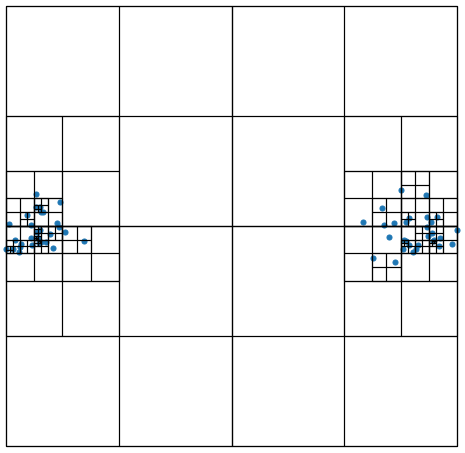
\includegraphics[width=1\textwidth]{figuras/expertos/tsne/quadtree.png}
        \caption{}
    \end{subfigure}
    \hspace{5em}
    \begin{subfigure}{.3\textwidth}
        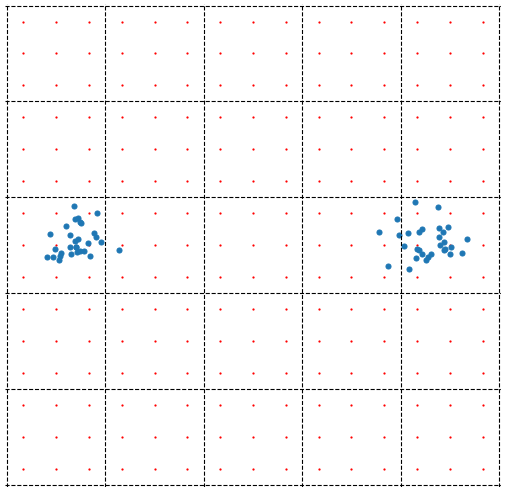
\includegraphics[width=1\textwidth]{figuras/expertos/tsne/interpolation_grid.png}
        \caption{}
    \end{subfigure}
    \caption{ Métodos aproximados para el cálculo de interacciones entre puntos. (a) Partición obtenida mediante un árbol cuaternario (\textit{quadtree}) (Aproximación Barnes-Hut). (b) Grilla de interpolación (puntos rojos equiespaciados en el plano).}
    \label{fig:tsne_approx}
\end{figure}

\section{Técnicas de optimización}\label{sec:tsne_optim}

Finalmente es importante mencionar que existen diferentes esquemas de optimización de mapeos t-SNE donde el parámetro de exageración $\varepsilon^{(n)}$ varía según la iteración $n$ en la que nos encontremos. En general, las implementaciones de t-SNE utilizan un valor por defecto de $\varepsilon^{(n)} = 12$ en las primeras 250 iteraciones, para luego fijar $\varepsilon^{(n)} = 1$ hasta el final de la optimización \cite{kobak_art}. Este procedimiento fue descripto por van der Maaten y Hinton junto con su introducción del algoritmo t-SNE en 2008 \cite{vdm_tsne}, y se denomina exageración temprana (\textit{early exaggertaion}). Al aumentar drásticamente el valor del factor de exageración, durante las primeras iteraciones del proceso de optimización, se le da un peso importante al término atractivo del gradiente de la función de costo. Para contrarrestar este desequilibrio del término de los $p_{ij}$ (el cual es el término atractivo del gradiente), el término repulsivo responde intentando aumentar los valores de los $q_{ij}$. Como resultado se fomenta la formación de \textit{clusters} muy densos y separados entre sí en el espacio de salida. En consecuencia, esto crea relativamente mucho espacio vacío en el espacio de salida, lo cual facilita el reacomodamiento de \textit{clusters} durante el resto del proceso de optimización \cite{vdm_tsne}.

Dentro del esquema de exageración temprana, suele utilizarse además un esquema de exageración tardía (\textit{late exaggertaion}) \cite{kobak_art, linderman_tsne}. Esta vez, se aumenta el valor del factor de exageración durante las últimas iteraciones del proceso de optimización. Esto produce un mapeo t-SNE final con \textit{clusters} más densos y con mayor separación entre sí, facilitando en última instancia la segmentación de los mismos.

La Figura \ref{fig:alpha_late} muestra diferentes mapas t-SNE obtenidos a partir de un conjunto de datos sintéticos, para diferentes valores de parámetro $\alpha$ (diferentes grados de libertad del \textit{kernel} t de Student), según se utilice o no exageración tardía. Todos estos mapas fueron obtenidos utilizando exageración temprana con $\varepsilon = 12$ durante las primeras 250 iteraciones, y el proceso de optimización comprendió un total de 1000 iteraciones. En caso de utilizar además exageración tardía, esta consistió en las últimas 50 iteraciones con $\varepsilon = 2$. Los datos sintéticos consistieron en 10 nubes gaussianas, de 100 puntos cada una, en un espacio de 20 dimensiones, con desviación estándar $\sigma = 1$ y medias aleatorias. Para cada una de estas nubes, 50 puntos se desplazaron en $2\vb{e}_{10+l}$ y los otros 50 puntos restantes en $-2\vb{e}_{10+l}$, donde $l$ es el número de clase de la nube y $\vb{e}_j$ es el $j$-ésimo vector unitario del espacio de 20 dimensiones. De esta manera se deforman las nubes gaussianas y se les da forma de mancuerna. Note que utilizar un parámetro de grados de libertad $\alpha=100$ equivale aproximadamente a utilizar un \textit{kernel} gaussiano en el espacio de salida, como se hacía originalmente en el algoritmo SNE. Por otro lado $\alpha=1$ corresponde implementación usual de t-SNE y $\alpha<1$ corresponde a distribuciones con colas más pesadas aún. En consecuencia el parámetro $\alpha$, en conjunto con el esquema de exageración tardía, pueden utilizarse para obtener diversos mapeos t-SNE de un mismo conjunto de datos, según nuestra intención sea la visualización de estos datos o la segmentación de los datos en \textit{clusters} bien definidos.

\begin{figure}[!htbp]
\begin{tabular}{cccc}
\centering
 & $\alpha = 100$ & $\alpha = 1$ & $\alpha = 0.5$ \\
\rotatebox[origin=c]{90}{Sin exag. tardía} & \raisebox{-0.5\height}{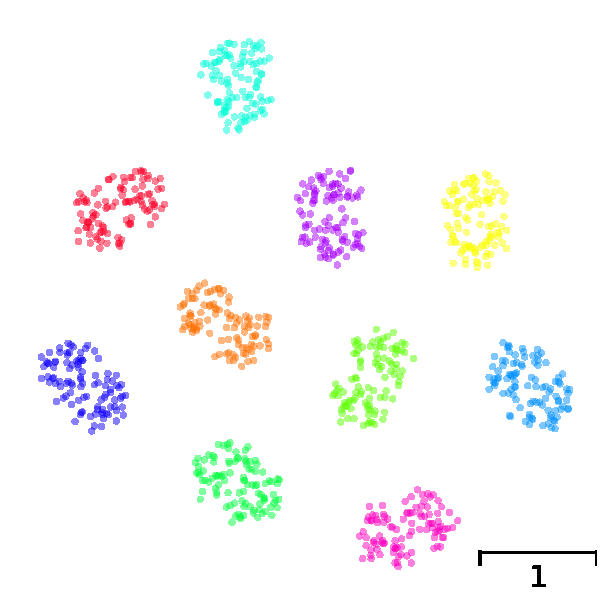
\includegraphics[width=0.27\textwidth]{figuras/expertos/tsne/tsne_alpha100_exaggs(12, 1, 1).pdf}} & \raisebox{-0.5\height}{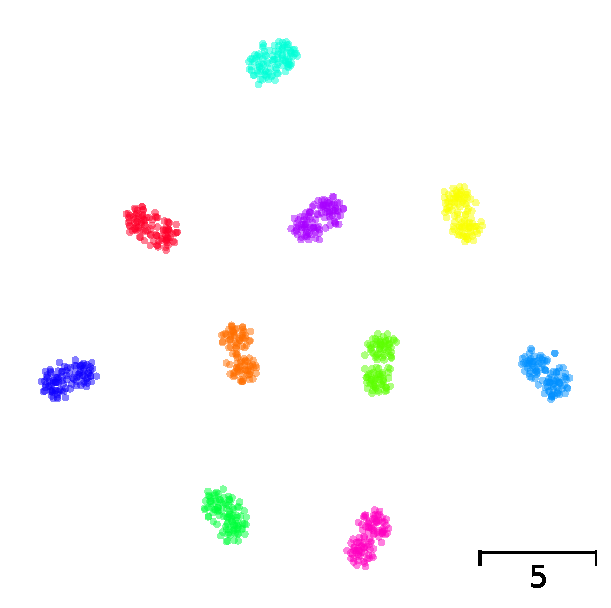
\includegraphics[width=0.27\textwidth]{figuras/expertos/tsne/tsne_alpha1_exaggs(12, 1, 1).pdf}} & \raisebox{-0.5\height}{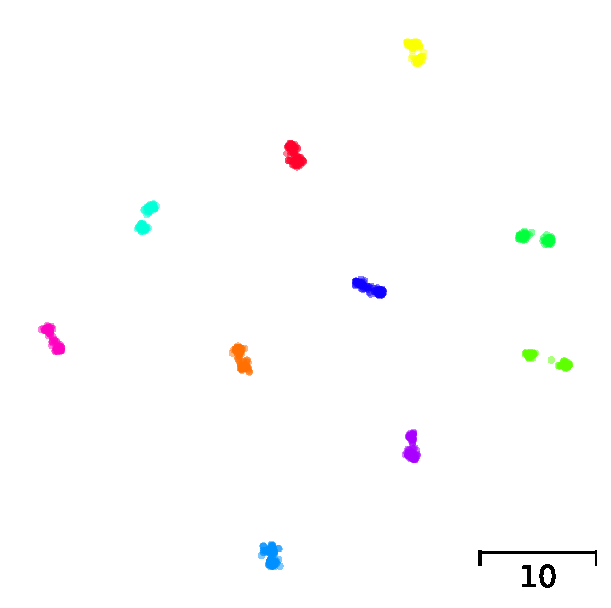
\includegraphics[width=0.27\textwidth]{figuras/expertos/tsne/tsne_alpha0.5_exaggs(12, 1, 1).pdf}} \\
\rotatebox[origin=c]{90}{Con exag. tardía} & \raisebox{-0.5\height}{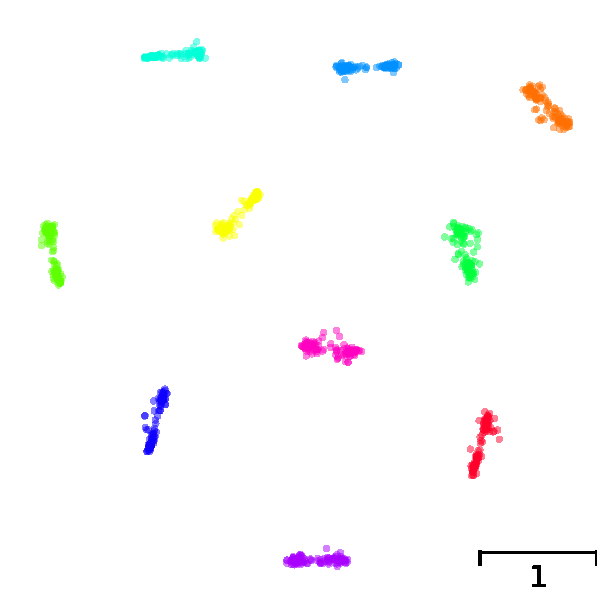
\includegraphics[width=0.27\textwidth]{figuras/expertos/tsne/tsne_alpha100_exaggs(12, 1, 2).pdf}} & \raisebox{-0.5\height}{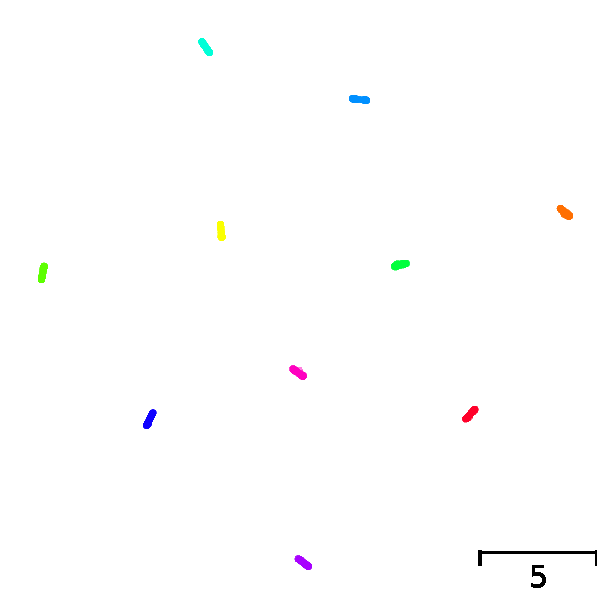
\includegraphics[width=0.27\textwidth]{figuras/expertos/tsne/tsne_alpha1_exaggs(12, 1, 2).pdf}} & \raisebox{-0.5\height}{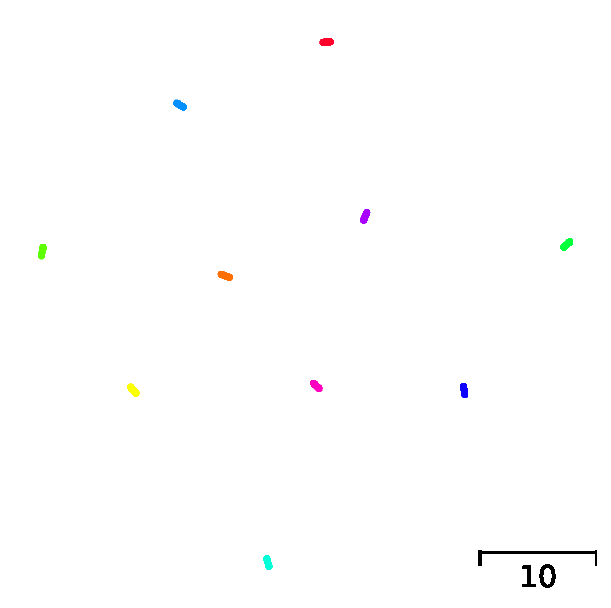
\includegraphics[width=0.27\textwidth]{figuras/expertos/tsne/tsne_alpha0.5_exaggs(12, 1, 2).pdf}}
\end{tabular}
\caption{Comparación de los efectos de utilizar diferentes parámetros o esquemas de optimización del algoritmo t-SNE sobre un conjunto de datos sintéticos: diferentes grados de libertad $\alpha$ en el \textit{kernel} t de Student del espacio de salida del mapeo t-SNE y utilización o no de esquema de exageración tardía durante el proceso de optimización.}
\label{fig:alpha_late}
\end{figure}

\section{Parámetros utilizados en el mapa de comportamientos}\label{sec:tsne_param}

La Tabla \ref{tab:tsne_param} muestra los valores de los parámetros utilizados en el algoritmo t-SNE para la obtención del mapa de comportamientos de la Figura \ref{fig:tsne_black}. Note que el proceso de optimización de un mapa t-SNE puede dividirse en 3 etapas: temprana, regular y tardía, que pueden comprender diferentes cantidades de iteraciones ($n_{\mathrm{iter}}$) y durante las cuales por lo general varía el valor del factor de exageración ($\varepsilon$). Los demás parámetros del algoritmo t-SNE que no se mencionan en la Tabla \ref{tab:tsne_param} se fijaron en sus valores por defecto en la implementación de \texttt{openTSNE} \cite{policar_tsne}.

\begin{table}[!htbp]
\begin{tabular}{lcccc}
\textbf{Etapa} & \textbf{Exag.} ($\varepsilon$) & \textbf{Iteraciones} ($n_{\mathrm{iter}}$) & \textbf{Perp.} ($\mathcal{P}$) & \textbf{Grados de libertad} ($\alpha$) \\ \hline
Temprana & 12 & 250 & 30 & 0.4 \\
Regular & 5 & 750 & 30 & 0.4 \\
Tardía & 10 & 750 & 30 & 0.4 \\
\end{tabular}
\caption{ Parámetros utilizados durante la ejecución del algoritmo t-SNE mediante el cual se obtuvo el etograma de la Figura \ref{fig:tsne_black}.}
\label{tab:tsne_param}
\end{table}

\chapter{Patrones de actividad de grupos de neuronas, continuación}\label{cha:popu_cont}

Las Figuras \ref{fig:zscore_label1}, \ref{fig:zscore_label3}, \ref{fig:zscore_label4}, \ref{fig:zscore_label8} y \ref{fig:zscore_label9} muestran los patrones de actividad de grupos de neuronas ante la ocurrencia de eventos de \textit{onset} y \textit{offset} de los \textit{labels} 1, 3, 4, 8 y 9, respectivamente. Cada fila en los \textit{heatmaps} representa una neurona individual. El tiempo de ocurrencia del evento se indica con una línea discontinua negra. Además, estos \textit{heatmaps} presentan una división entre neuronas no moduladas y moduladas ante la ocurrencia del evento de transición (línea continua negra). A su vez, cada uno de estos grupos de neuronas se ordena de tres maneras diferentes para facilitar su visualización: pueden estar ordenados según la posición del máximo o del mínimo de su \textit{z-score} o según un orden por defecto.

\begin{figure}[!htbp]
\begin{tabular}{clll}
& & \multicolumn{2}{c}{\hspace{-5.5em} \textit{label} 1} \\
& & \hspace{6em} \textit{Onset} & \hspace{6em} \textit{Offset} \\
\rotatebox[origin=c]{90}{Orden según máximo} & \rotatebox{90}{\hspace{-8.5em} Moduladas \hspace{2.5em} No moduladas} & \raisebox{-0.5\height}{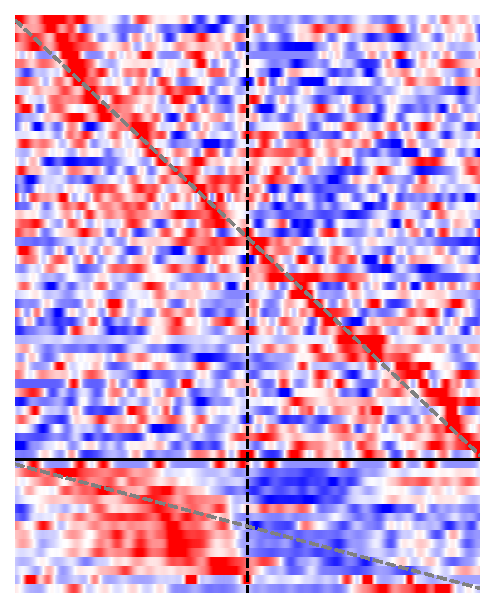
\includegraphics[width=0.37\textwidth]{figuras/expertos/zscore/rasters_separate_days_zscore_max_onset_label1.pdf}} &
\raisebox{-0.5\height}{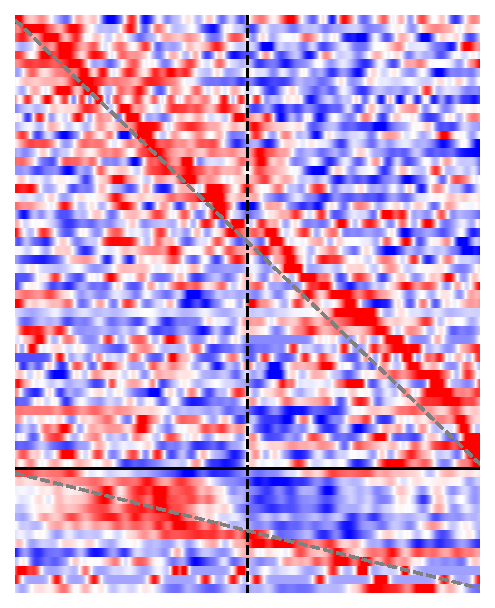
\includegraphics[width=0.37\textwidth]{figuras/expertos/zscore/rasters_separate_days_zscore_max_offset_label1.pdf}} \\
\rotatebox[origin=c]{90}{Orden según mínimo} & & \raisebox{-0.5\height}{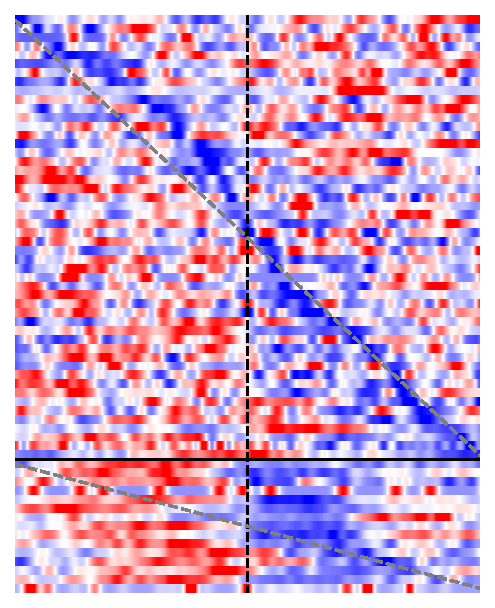
\includegraphics[width=0.37\textwidth]{figuras/expertos/zscore/rasters_separate_days_zscore_min_onset_label1.pdf}} &
\raisebox{-0.5\height}{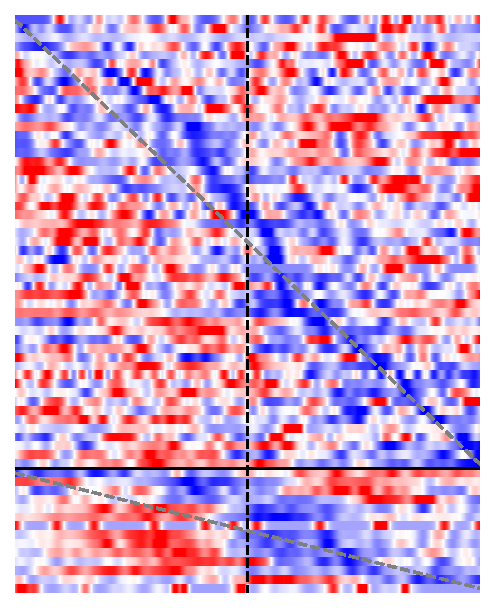
\includegraphics[width=0.37\textwidth]{figuras/expertos/zscore/rasters_separate_days_zscore_min_offset_label1.pdf}} \\
\rotatebox{90}{Orden por defecto} & & \hspace{-1.5em} \raisebox{-0.5\height}{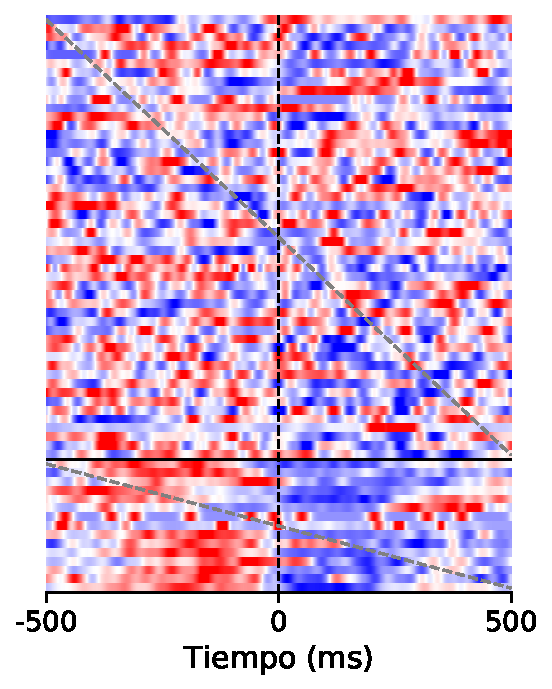
\includegraphics[width=0.42\textwidth]{figuras/expertos/zscore/rasters_separate_days_zscore_deafult_onset_label1.pdf}} & \hspace{-1.3em} \raisebox{-0.495\height}{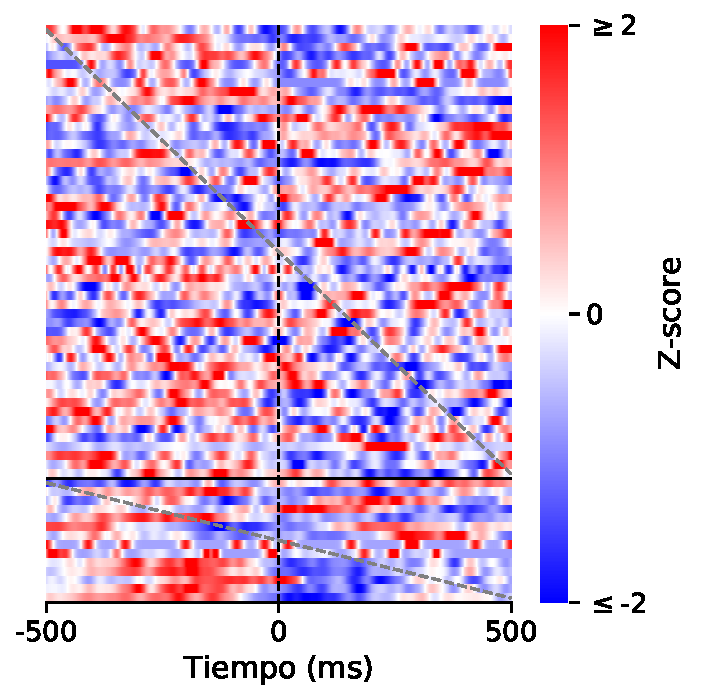
\includegraphics[width=0.53\textwidth]{figuras/expertos/zscore/rasters_separate_days_zscore_deafult_offset_label1.pdf}}
\end{tabular}
\caption{\textit{Heatmaps} con las respuestas de grupos de neuronas ante la ocurrencia de eventos de transición que involucran al \textit{label} 1. Cada fila de un \textit{heatmap} representa el \textit{z-score} de una única neurona. La actividad de las neuronas están divididas en no moduladas y moduladas. Las actividades de las neuronas se ordenan según la posición de su máximo, mínimo y según un orden por defecto.}
\label{fig:zscore_label1}
\end{figure}

\begin{figure}[!htbp]
\begin{tabular}{clll}
& & \multicolumn{2}{c}{\hspace{-5.5em} \textit{label} 3} \\
& & \hspace{6em} \textit{Onset} & \hspace{6em} \textit{Offset} \\
\rotatebox[origin=c]{90}{Orden según máximo} & \rotatebox{90}{\hspace{-8.5em} Moduladas \hspace{2.5em} No moduladas} & \raisebox{-0.5\height}{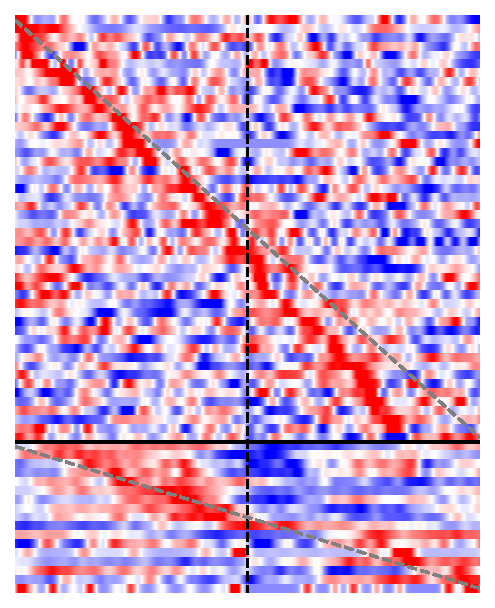
\includegraphics[width=0.37\textwidth]{figuras/expertos/zscore/rasters_separate_days_zscore_max_onset_label3.pdf}} &
\raisebox{-0.5\height}{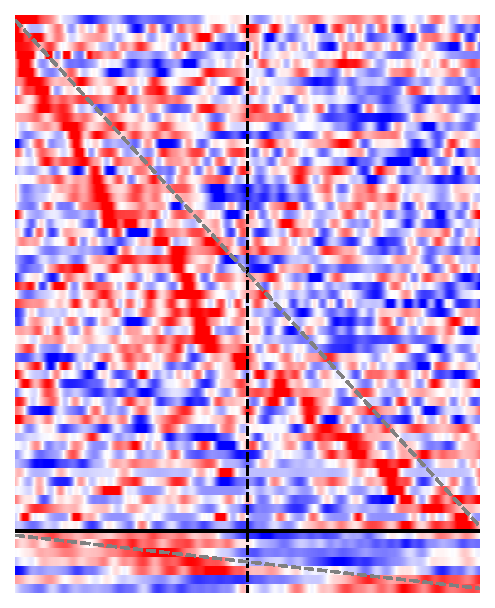
\includegraphics[width=0.37\textwidth]{figuras/expertos/zscore/rasters_separate_days_zscore_max_offset_label3.pdf}} \\
\rotatebox[origin=c]{90}{Orden según mínimo} & & \raisebox{-0.5\height}{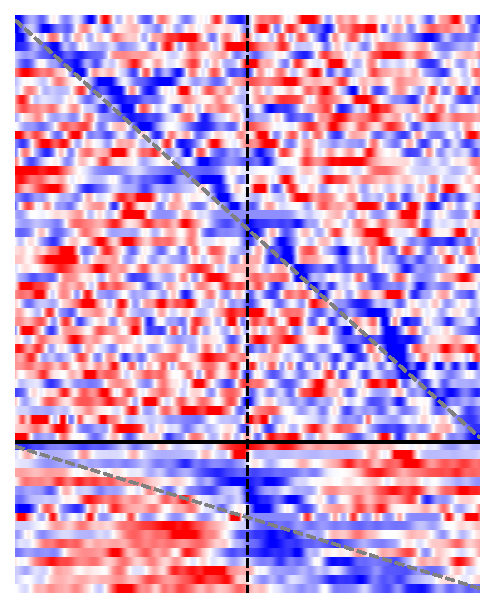
\includegraphics[width=0.37\textwidth]{figuras/expertos/zscore/rasters_separate_days_zscore_min_onset_label3.pdf}} &
\raisebox{-0.5\height}{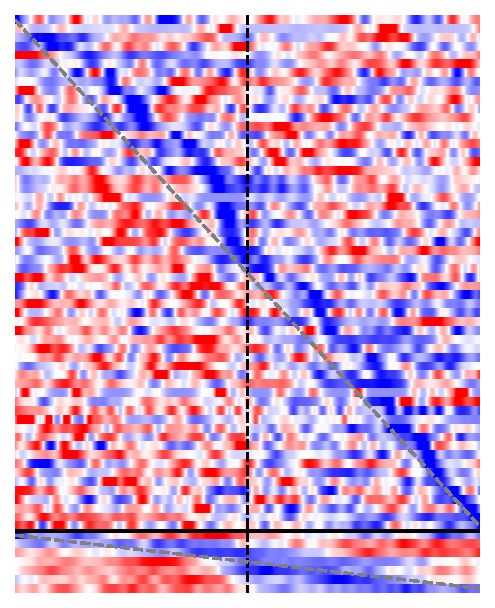
\includegraphics[width=0.37\textwidth]{figuras/expertos/zscore/rasters_separate_days_zscore_min_offset_label3.pdf}} \\
\rotatebox{90}{Orden por defecto} & & \hspace{-1.5em} \raisebox{-0.5\height}{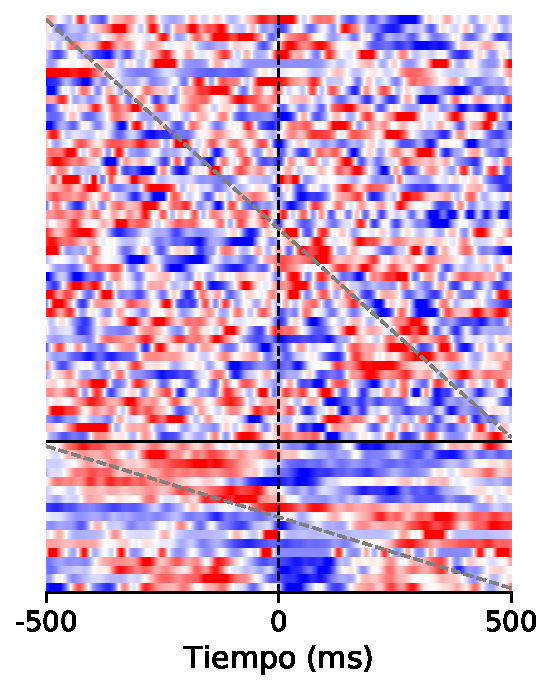
\includegraphics[width=0.42\textwidth]{figuras/expertos/zscore/rasters_separate_days_zscore_deafult_onset_label3.pdf}} & \hspace{-1.3em} \raisebox{-0.495\height}{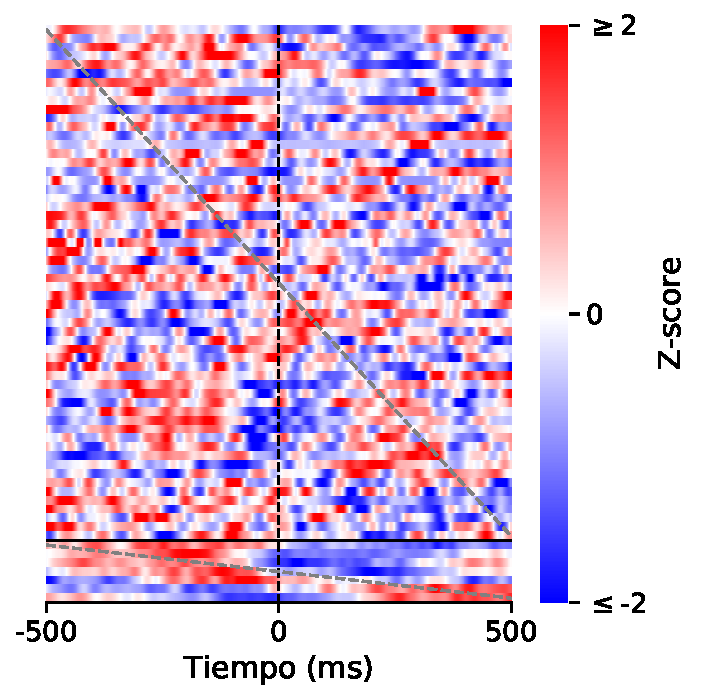
\includegraphics[width=0.53\textwidth]{figuras/expertos/zscore/rasters_separate_days_zscore_deafult_offset_label3.pdf}}
\end{tabular}
\caption{\textit{Heatmaps} con las respuestas de grupos de neuronas ante la ocurrencia de eventos de transición que involucran al \textit{label} 3. Cada fila de un \textit{heatmap} representa el \textit{z-score} de una única neurona. La actividad de las neuronas están divididas en no moduladas y moduladas. Las actividades de las neuronas se ordenan según la posición de su máximo, mínimo y según un orden por defecto.}
\label{fig:zscore_label3}
\end{figure}

\begin{figure}[!htbp]
\begin{tabular}{clll}
& & \multicolumn{2}{c}{\hspace{-5.5em} \textit{label} 4} \\
& & \hspace{6em} \textit{Onset} & \hspace{6em} \textit{Offset} \\
\rotatebox[origin=c]{90}{Orden según máximo} & \rotatebox{90}{\hspace{-8.5em} Moduladas \hspace{2.5em} No moduladas} & \raisebox{-0.5\height}{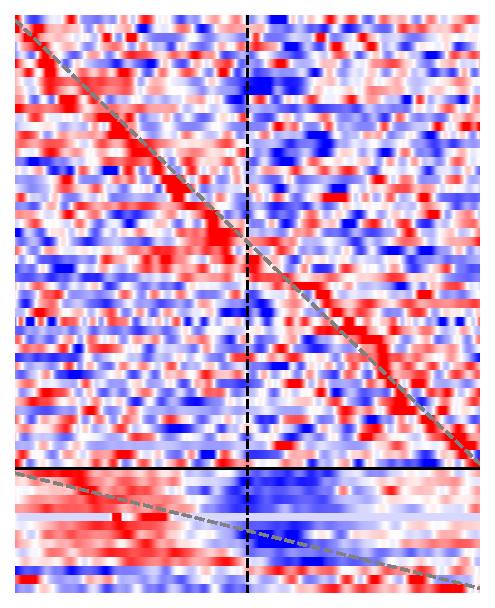
\includegraphics[width=0.37\textwidth]{figuras/expertos/zscore/rasters_separate_days_zscore_max_onset_label4.pdf}} &
\raisebox{-0.5\height}{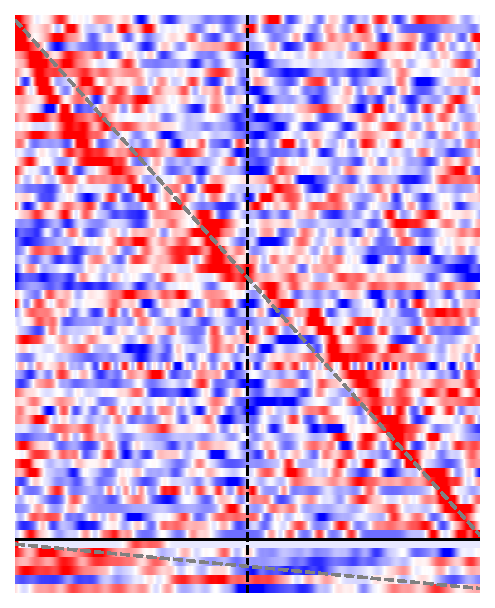
\includegraphics[width=0.37\textwidth]{figuras/expertos/zscore/rasters_separate_days_zscore_max_offset_label4.pdf}} \\
\rotatebox[origin=c]{90}{Orden según mínimo} & & \raisebox{-0.5\height}{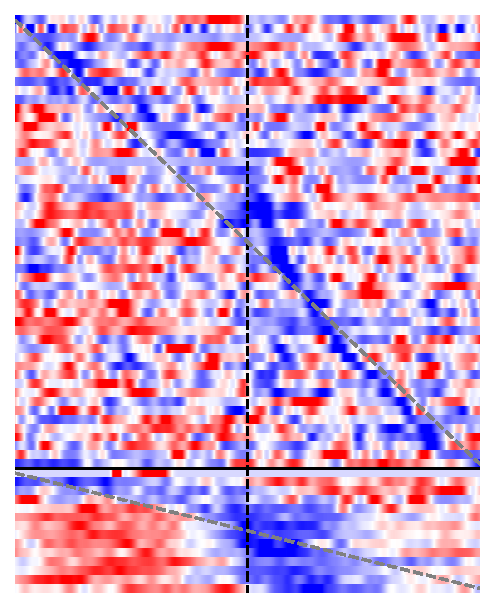
\includegraphics[width=0.37\textwidth]{figuras/expertos/zscore/rasters_separate_days_zscore_min_onset_label4.pdf}} &
\raisebox{-0.5\height}{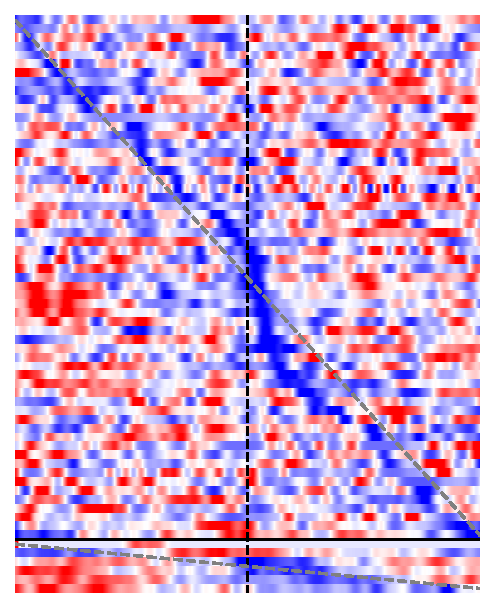
\includegraphics[width=0.37\textwidth]{figuras/expertos/zscore/rasters_separate_days_zscore_min_offset_label4.pdf}} \\
\rotatebox{90}{Orden por defecto} & & \hspace{-1.5em} \raisebox{-0.5\height}{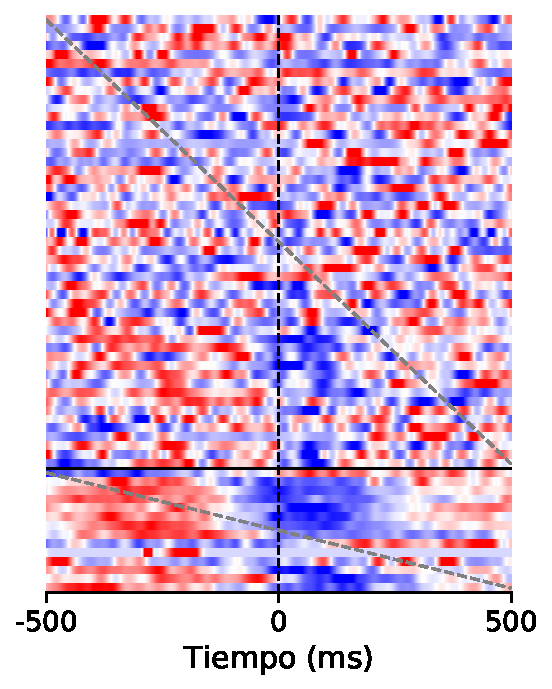
\includegraphics[width=0.42\textwidth]{figuras/expertos/zscore/rasters_separate_days_zscore_deafult_onset_label4.pdf}} & \hspace{-1.3em} \raisebox{-0.495\height}{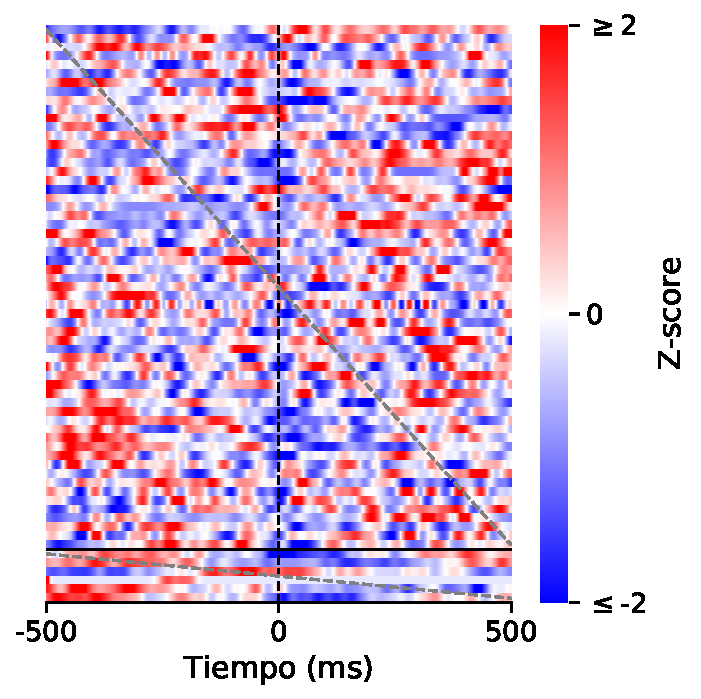
\includegraphics[width=0.53\textwidth]{figuras/expertos/zscore/rasters_separate_days_zscore_deafult_offset_label4.pdf}}
\end{tabular}
\caption{\textit{Heatmaps} con las respuestas de grupos de neuronas ante la ocurrencia de eventos de transición que involucran al \textit{label} 4. Cada fila de un \textit{heatmap} representa el \textit{z-score} de una única neurona. La actividad de las neuronas están divididas en no moduladas y moduladas. Las actividades de las neuronas se ordenan según la posición de su máximo, mínimo y según un orden por defecto.}
\label{fig:zscore_label4}
\end{figure}

\begin{figure}[!htbp]
\begin{tabular}{clll}
& & \multicolumn{2}{c}{\hspace{-5.5em} \textit{label} 8} \\
& & \hspace{6em} \textit{Onset} & \hspace{6em} \textit{Offset} \\
\rotatebox[origin=c]{90}{Orden según máximo} & \rotatebox{90}{\hspace{-8.5em} Moduladas \hspace{2.5em} No moduladas} & \raisebox{-0.5\height}{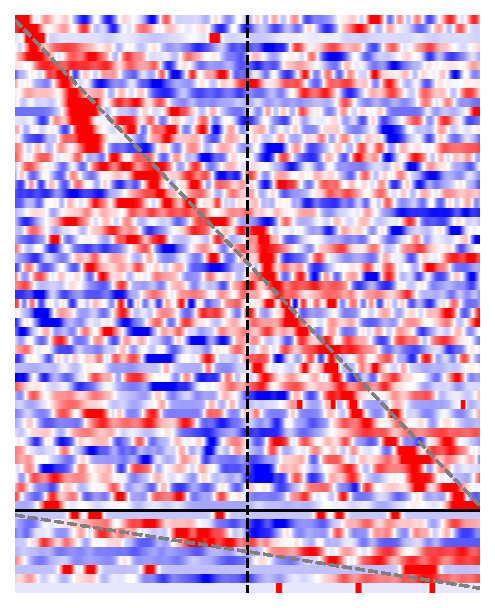
\includegraphics[width=0.37\textwidth]{figuras/expertos/zscore/rasters_separate_days_zscore_max_onset_label8.pdf}} &
\raisebox{-0.5\height}{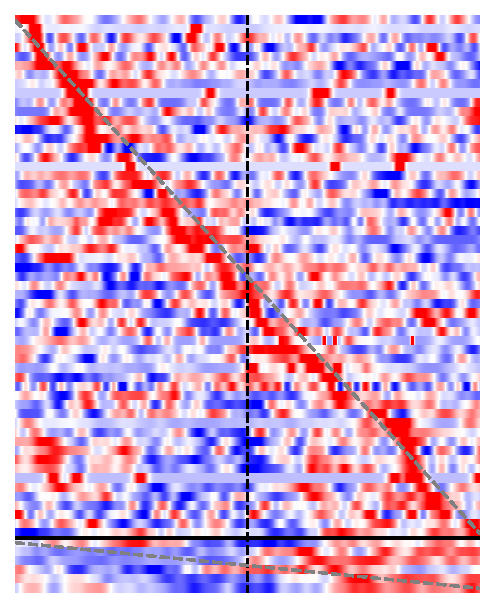
\includegraphics[width=0.37\textwidth]{figuras/expertos/zscore/rasters_separate_days_zscore_max_offset_label8.pdf}} \\
\rotatebox[origin=c]{90}{Orden según mínimo} & & \raisebox{-0.5\height}{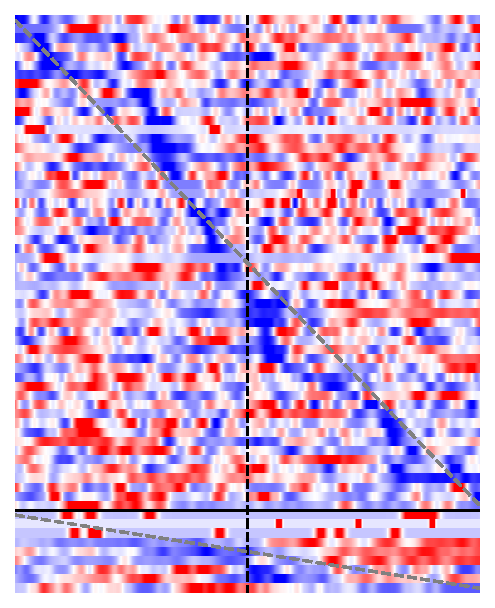
\includegraphics[width=0.37\textwidth]{figuras/expertos/zscore/rasters_separate_days_zscore_min_onset_label8.pdf}} &
\raisebox{-0.5\height}{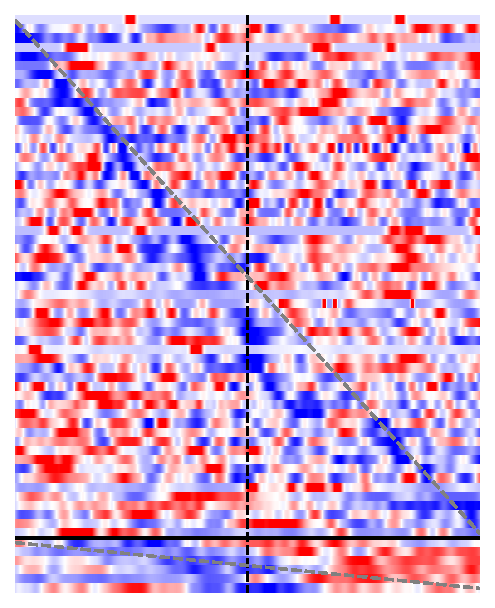
\includegraphics[width=0.37\textwidth]{figuras/expertos/zscore/rasters_separate_days_zscore_min_offset_label8.pdf}} \\
\rotatebox{90}{Orden por defecto} & & \hspace{-1.5em} \raisebox{-0.5\height}{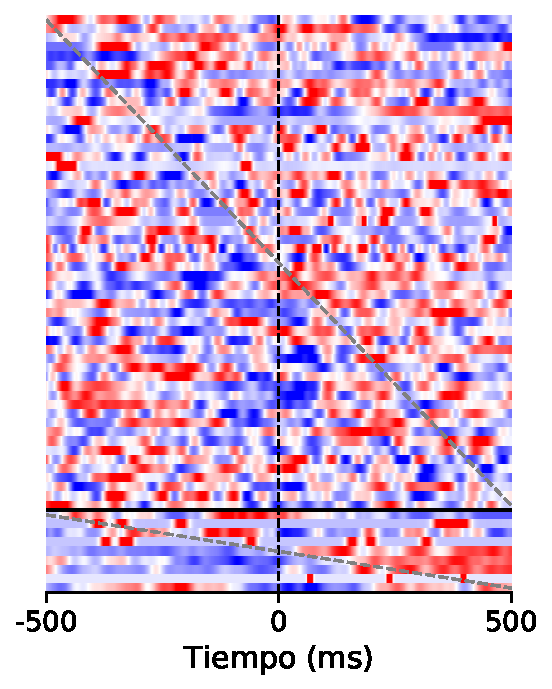
\includegraphics[width=0.42\textwidth]{figuras/expertos/zscore/rasters_separate_days_zscore_deafult_onset_label8.pdf}} & \hspace{-1.3em} \raisebox{-0.495\height}{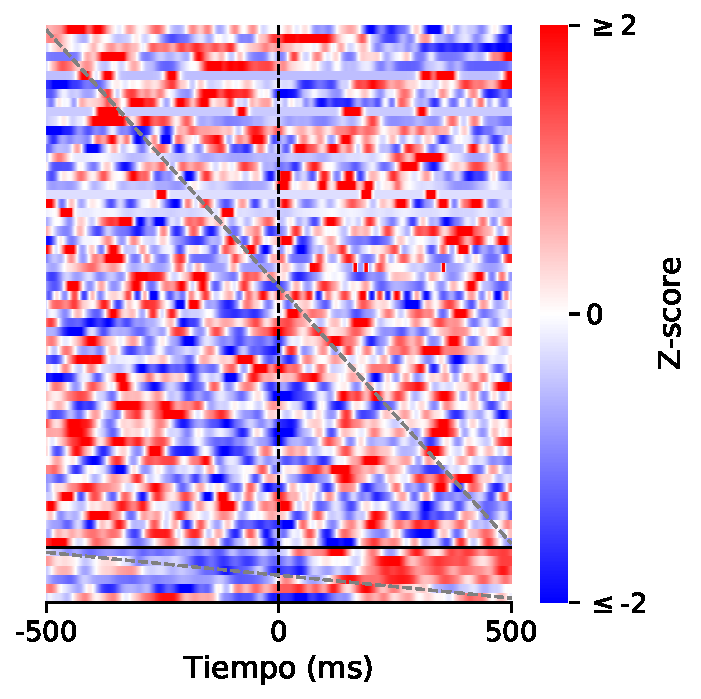
\includegraphics[width=0.53\textwidth]{figuras/expertos/zscore/rasters_separate_days_zscore_deafult_offset_label8.pdf}}
\end{tabular}
\caption{\textit{Heatmaps} con las respuestas de grupos de neuronas ante la ocurrencia de eventos de transición que involucran al \textit{label} 8. Cada fila de un \textit{heatmap} representa el \textit{z-score} de una única neurona. La actividad de las neuronas están divididas en no moduladas y moduladas. Las actividades de las neuronas se ordenan según la posición de su máximo, mínimo y según un orden por defecto.}
\label{fig:zscore_label8}
\end{figure}

\begin{figure}[!htbp]
\begin{tabular}{clll}
& & \multicolumn{2}{c}{\hspace{-5.5em} \textit{label} 9} \\
& & \hspace{6em} \textit{Onset} & \hspace{6em} \textit{Offset} \\
\rotatebox[origin=c]{90}{Orden según máximo} & \rotatebox{90}{\hspace{-8.5em} Moduladas \hspace{2.5em} No moduladas} & \raisebox{-0.5\height}{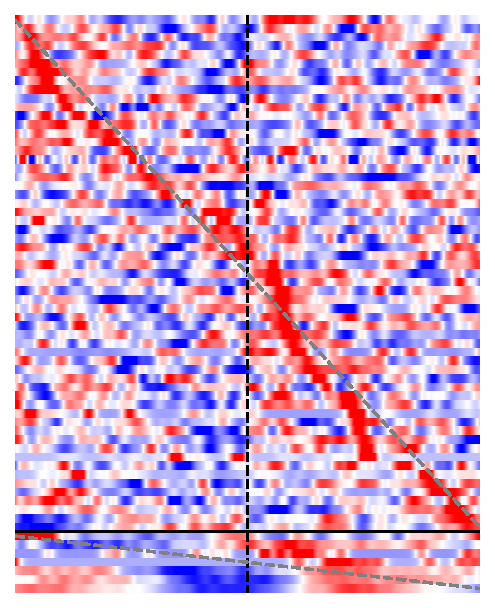
\includegraphics[width=0.37\textwidth]{figuras/expertos/zscore/rasters_separate_days_zscore_max_onset_label9.pdf}} &
\raisebox{-0.5\height}{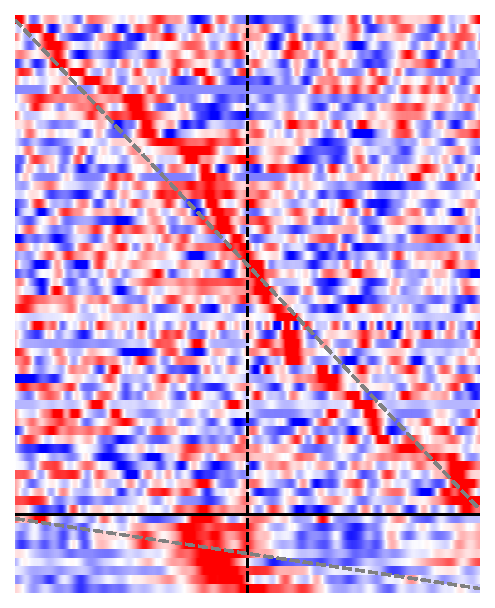
\includegraphics[width=0.37\textwidth]{figuras/expertos/zscore/rasters_separate_days_zscore_max_offset_label9.pdf}} \\
\rotatebox[origin=c]{90}{Orden según mínimo} & & \raisebox{-0.5\height}{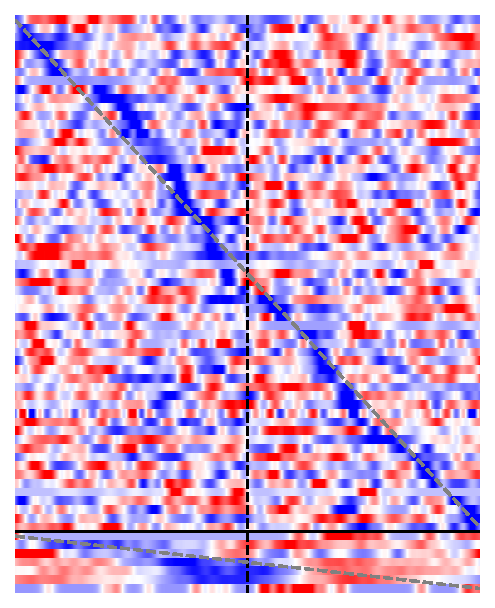
\includegraphics[width=0.37\textwidth]{figuras/expertos/zscore/rasters_separate_days_zscore_min_onset_label9.pdf}} &
\raisebox{-0.5\height}{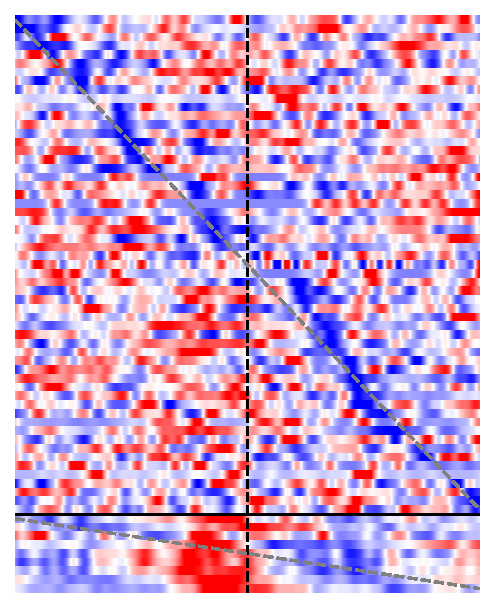
\includegraphics[width=0.37\textwidth]{figuras/expertos/zscore/rasters_separate_days_zscore_min_offset_label9.pdf}} \\
\rotatebox{90}{Orden por defecto} & & \hspace{-1.5em} \raisebox{-0.5\height}{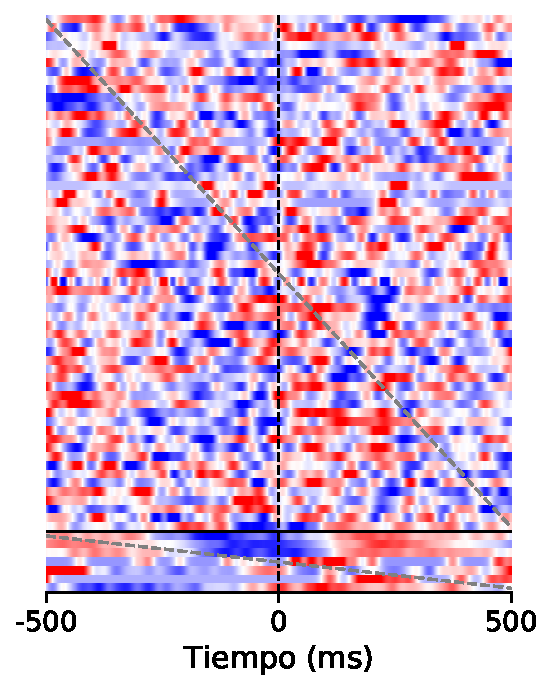
\includegraphics[width=0.42\textwidth]{figuras/expertos/zscore/rasters_separate_days_zscore_deafult_onset_label9.pdf}} & \hspace{-1.3em} \raisebox{-0.495\height}{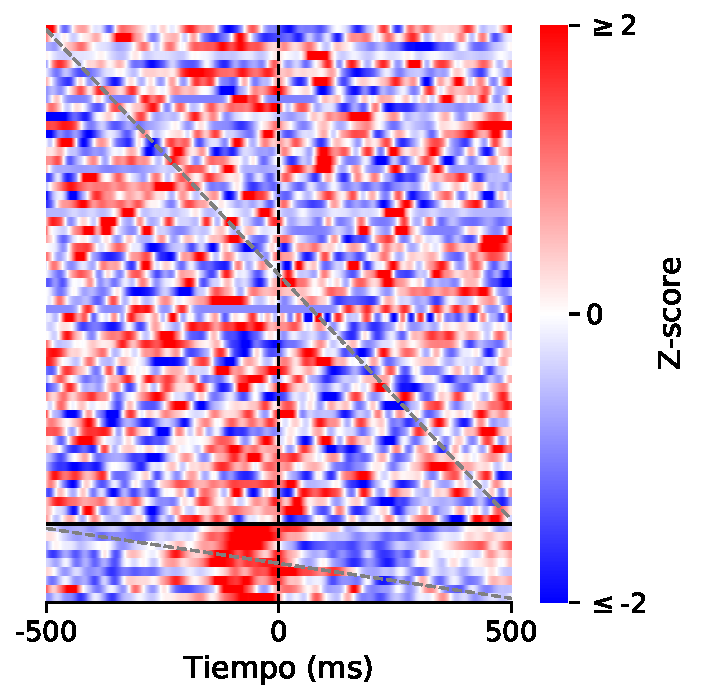
\includegraphics[width=0.53\textwidth]{figuras/expertos/zscore/rasters_separate_days_zscore_deafult_offset_label9.pdf}}
\end{tabular}
\caption{\textit{Heatmaps} con las respuestas de grupos de neuronas ante la ocurrencia de eventos de transición que involucran al \textit{label} 9. Cada fila de un \textit{heatmap} representa el \textit{z-score} de una única neurona. La actividad de las neuronas están divididas en no moduladas y moduladas. Las actividades de las neuronas se ordenan según la posición de su máximo, mínimo y según un orden por defecto.}
\label{fig:zscore_label9}
\end{figure}